\section{Experiments}%
\label{sec:experiments}

We use a custom implementation in C++ of all algorithm.

We used almost the same setup of the first grid presented by \citeauthor{comp_mcts_mo}\cite{comp_mcts_mo}.
Only we considered one precise setup to compare multiple algorithms.
We consider a \gls{twm} problem on a \(8 \times 8\) grid. 
We consider \(2\) firefighter team.
The rewards of cells start at \(-1\) on the bottom left corner and increase by the by \(-1\) for each cell between a cell and the bottom left corner according to the manhattan distance.
Only neighbors cell can ignite each other with a probability of \(0.06\).
Firefighter teams have a \(0.8\) probability to extinguish any burning cell.
We then follow the following procedure to obtain a root state

\begin{enumerate}
    \item Initialize all the cells with \(66\) fuel. 
    \item Ignite the bottom left corner.
    \item Let the fire propagate with no cost for \(66\) turn.
    \item Scale down the amount of fuel on each cell by \(.06\) to avoid too long computation
\end{enumerate}

We use the same algorithm on \(100\) different root states, obtain by the previous procedure.
We then aggregate the results together to have an average value.
We used different algorithms:

\begin{itemize}
    \item random: select a random action among legal ones every turn.
    \item \gls{uct} with \(60\) seconds of search time and an exploration parameter \(c\) equal to 1.
    \item \gls{grave} with 60 seconds of search time, an \textit{bias}  of \(0.01\) and a \textit{ref} equal to 50.
    \item \gls{nrpa} with a root level 2 and 25 iterations per level.
    \item \gls{snrpa} with a root level 2 and 25 iterations per level and 100 playount at level 0.
\end{itemize}

All algortihms are rerun every turn, allowing us to use \gls{nrpa} by taking the first action in the returned sequence.
We also included a version of the \gls{snrpa} called \textit{srnpa\_os} which is not rerun every turn but run only once on the root state.
We then take the returned sequence and use it just like in a \gls{snrpa} playout.
This allow us to use the \gls{snrpa} with a level of 3 and 50 iteration per level with 100 playout at level 0 while still having a reasonable time of computation.

The figure \ref{fig:results} presents the aggragated results of a 100 run for each algorithm with the parameters presented before.
The blue and yellow bar shows respectively the average highest reward obtainable from the root state and the average lowest reward obtainable from the root state.
These two values are computed before running the algorithm by considering the best case scenario and the worst one.

\begin{figure}[htpb]
    \centering
    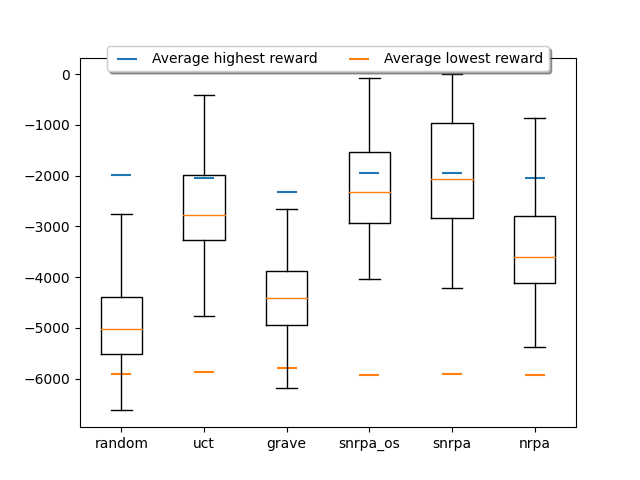
\includegraphics[width=0.8\linewidth]{./src/figures/moustache.png}
    \caption{Results on 100 simulation for different algorithm as described in section~\ref{sub:results} for different algorithms}
    \label{fig:results}
\end{figure}

The results show that the \gls{snrpa} performs significately better than other algorithm. 
We find strange that \gls{grave} algorithm performs so poorly and we extend the possibility of a non-wanted behaviour due to a code mistakes but we could not find one.
The \gls{nrpa} still performs better than the random algorithm which suggest that good sequences might be close to what the \gls{snrpa} find.

We wanted to see how the number of playout at level 0 impact the performance of the \gls{snrpa}.
We run, on the same setup as experiment 1 (see section~\ref{ssub:experiment_1}), 100 times the \gls{snrpa} with the same parameters.
Only one had 100 playout at level 0 and the other had 1000.

The results are shown in figure~\ref{fig:results_snrpa_playout}.
It shows that a bigger number of playouts tends to improve vastly the performance of the algorithm for a computation cost that does not increase that vastly.
The playout of the \gls{snrpa} are much simpler than the playout of the \gls{nrpa} and are computed much more faster.

\begin{figure}[htpb]
    \centering
    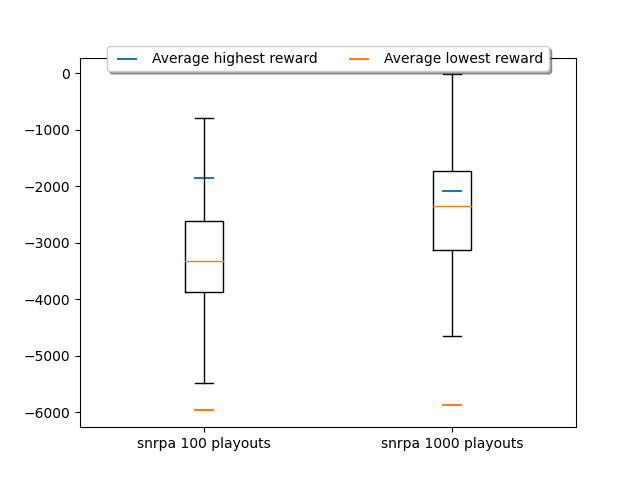
\includegraphics[width=0.8\linewidth]{./src/figures/moustache_snrpa.png}
    \caption{Comparison between a \gls{snrpa} with 100 playout at level 0 and a \gls{snrpa} with a 1000}
    \label{fig:results_snrpa_playout}
\end{figure}

The \gls{snrpa} seems to perform very well on this setup of grid.
It would be interesting to test it on other setup and problems, even on non stochastic ones where the \gls{nrpa} perform very well.
By lack of computational power and time we will most likely presents these tests later on another paper.

